\section{Polarizzazione}
Questa sezione ha come obiettivo quello di determinare la relazione tra intensità e angolo di polarizzazione.
Per condurre questa esperienza abbiamo disposto emettitore e ricevitore allineati e abbiamo ruotato il ricevitore di diversi angoli $\theta$.
Tenendo conto dell'imprecisione messa in evidenza nell'introduzione, abbiamo deciso di rappresentare la relazione in due modi differenti.
In primo luogo abbiamo utilizzato un'interpolazione lineare sul $\cos^2\vartheta$, verificando che l'apparato non avesse errore di calibrazione in base al verso della rotazione. I risultati sono riportati nella Figura \ref{polatizzazione fit quadratico}.
\begin{figure}[h!]
    \centering
    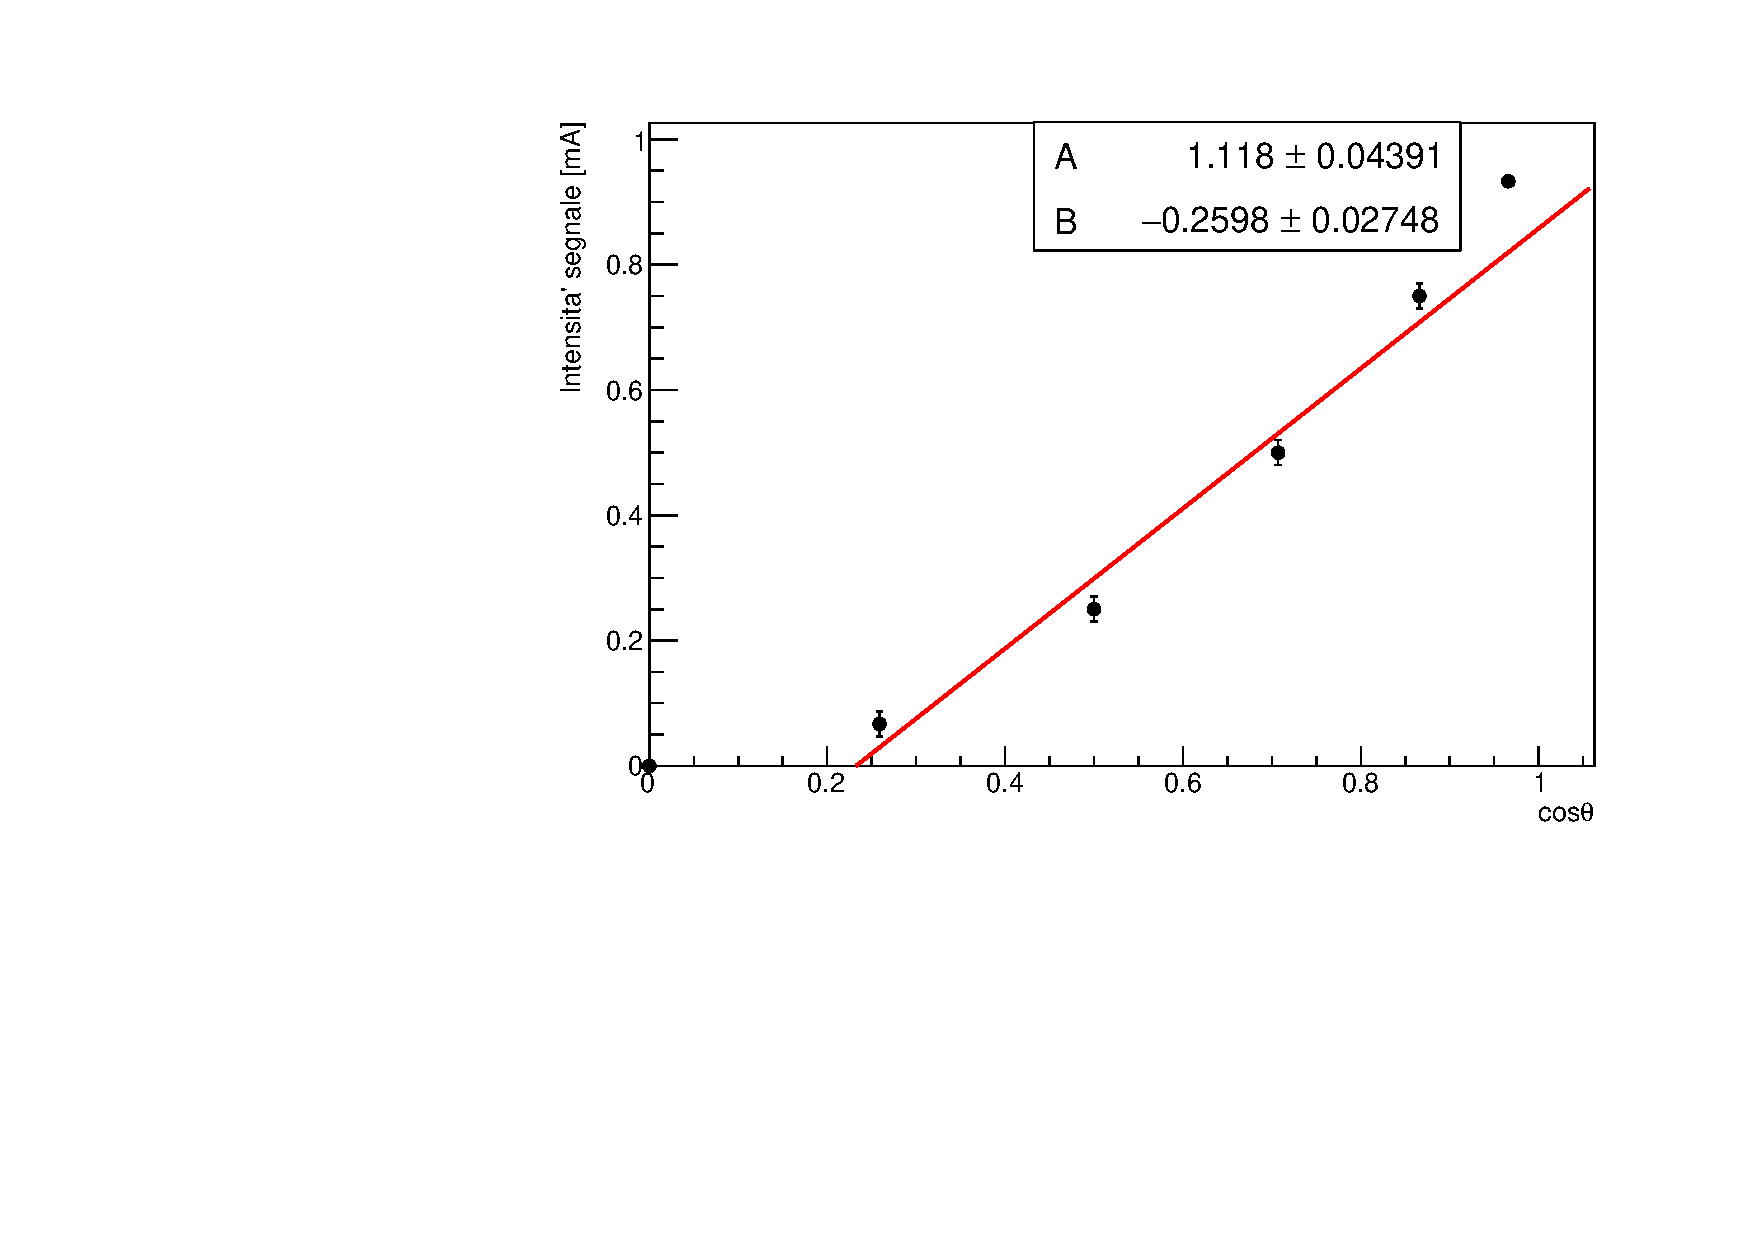
\includegraphics[scale=.5]{Immagini/coseni quadri lineare.pdf} 
    \caption{Interpolazione lineare}
    \label{polatizzazione fit quadratico}
\end{figure}
Abbiamo dimostrato questo mostrando come l'intensità fosse la medesima per angoli positivi e negativi di uguale modulo.

In secondo luogo abbiamo fatto uso di un'interpolazione quadratica che segue la legge di Malus, in grado di descrivere l'imprecisione sulla relazione tra il segnale rilevato e l'effettivo segnale trasmesso. Abbiamo interpolato seguendo 
$$
y=A\cos(\theta) + B(\cos^2\theta)
$$
dove per $y$ si considera il segnale misurato, il grafico è riportato nella Figura \ref{polatizzazione fit}.

\begin{figure}[h!]
    \centering
    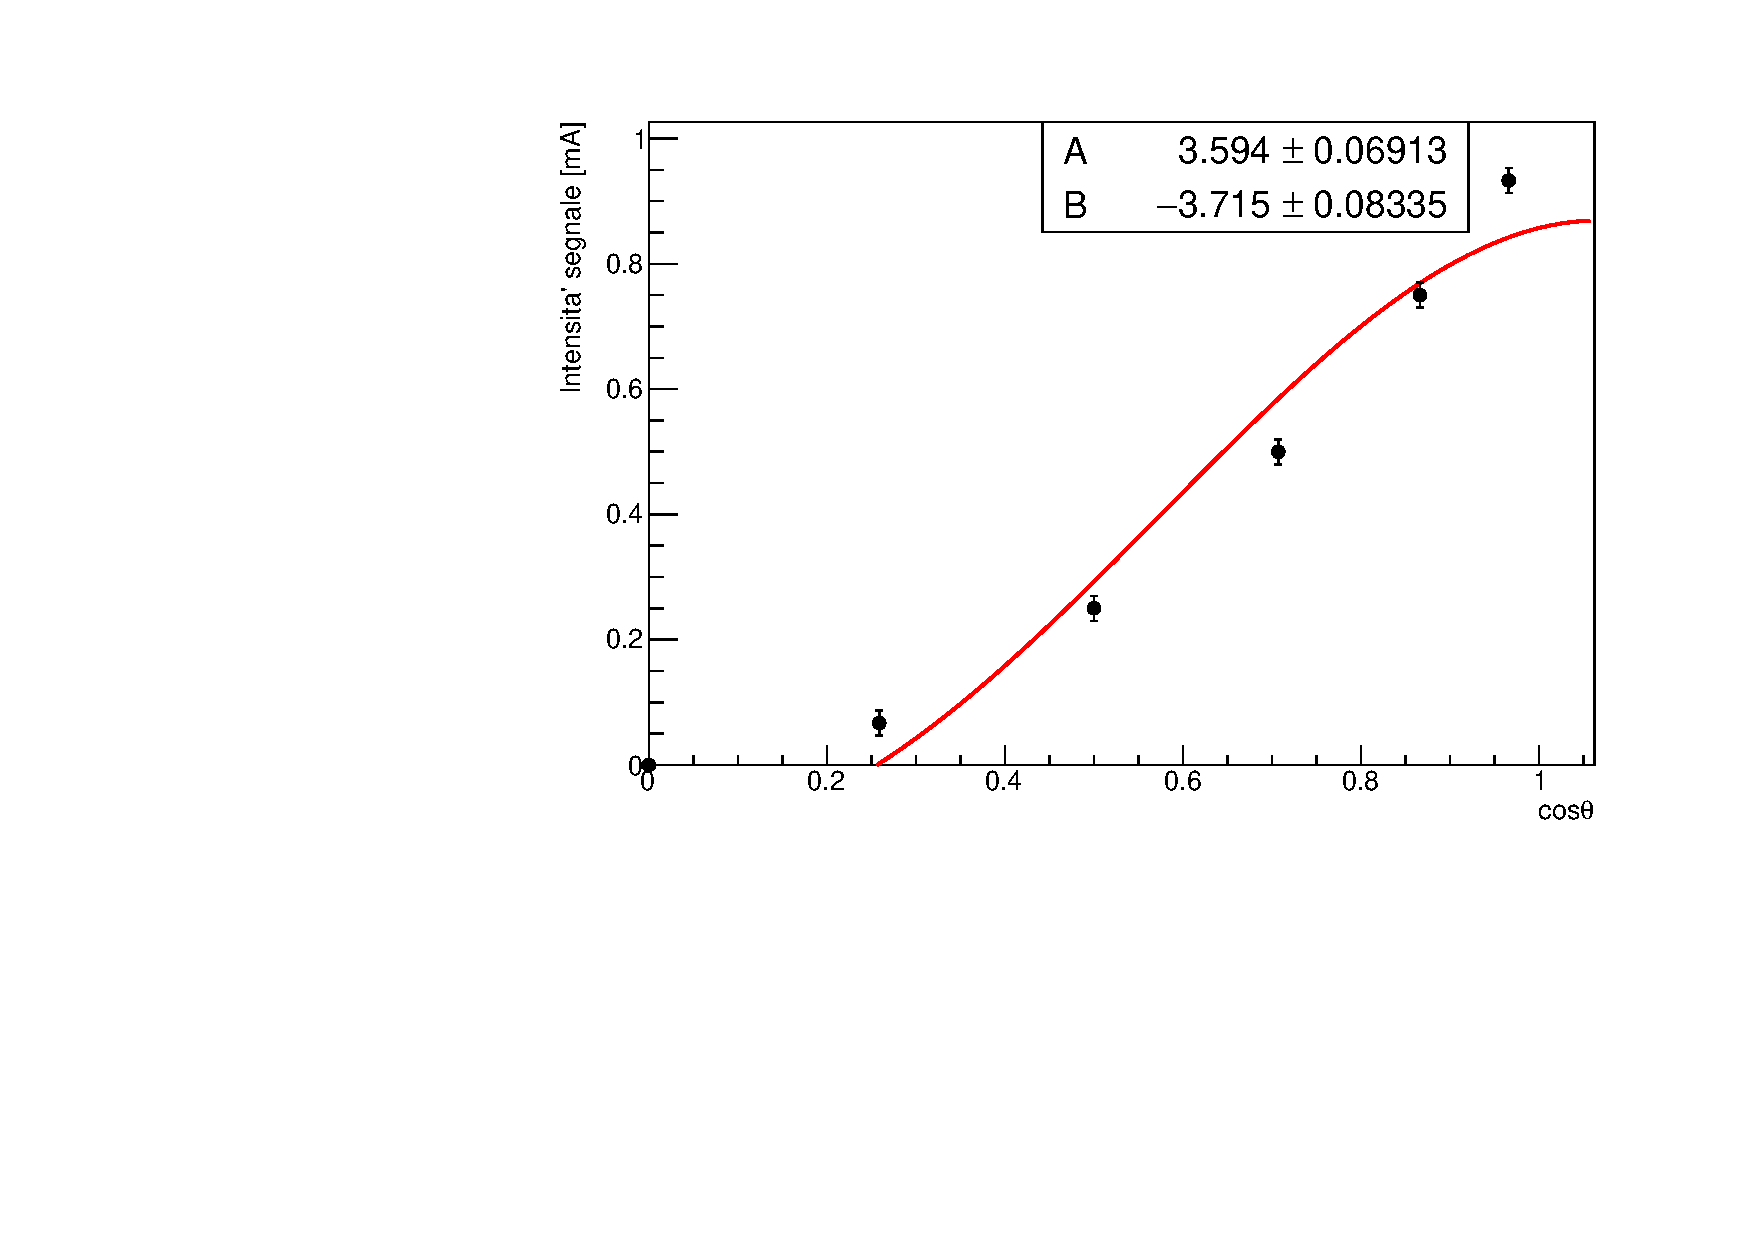
\includegraphics[scale=.5]{Immagini/coseni quadri.pdf}
    \caption{Interpolazione completa}
    \label{polatizzazione fit}
\end{figure}
Non essendo nota la relazione tra il segnale letto sul display dell'Amperometro e il valore medio del campo elettrico nel punto del ricevitore, abbiamo ipotizzato che questo avesse, nel primo caso, una dipendenza lineare dal campo, nel secondo caso, invece, una dipendenza "mista" sia dal campo che dall'intensità.
